\documentclass[11pt]{article}
\usepackage[a4paper,margin=20mm,headsep=6mm]{geometry}
\usepackage{amsmath,amssymb}
\usepackage[T1]{fontenc}
\usepackage{lmodern}
\usepackage{xcolor}
\usepackage{tikz}
\usetikzlibrary{arrows.meta}
\usepackage[most]{tcolorbox}
\usepackage{enumitem}
\usepackage{fancyhdr}
\usepackage{needspace}
\usepackage{lastpage}
\usepackage{environ}
\usepackage{array}
\usepackage{cancel}
\definecolor{chalk}{HTML}{2F6F8F}
\definecolor{chalkdk}{HTML}{24576F}
\definecolor{amber}{HTML}{D98A3D}
\definecolor{ink}{HTML}{1A2B34}
\definecolor{inksoft}{HTML}{4A5F68}
\definecolor{paper}{HTML}{F6F4EF}
\definecolor{line}{HTML}{DFE3E0}
\color{ink}
\setlength{\parindent}{0pt}
\setlength{\parskip}{4pt}
\setlength{\lineskiplimit}{2pt}\setlength{\lineskip}{4pt}
\pagestyle{fancy}
\fancyhf{}
\renewcommand{\headrulewidth}{0.4pt}
\renewcommand{\headrule}{\hbox to\headwidth{\color{line}\leaders\hrule height 0.4pt\hfill}}
\lhead{\small\color{inksoft}\textsc{Chapter 8 : Probability}}
\rhead{\small\color{inksoft}Year 10 Methods : Question Booklet}
\cfoot{\small\color{inksoft}Page \thepage\ of \pageref{LastPage}}
\newcommand{\sectionband}[3]{%
  \needspace{5\baselineskip}\vspace{6pt}
  \begin{tcolorbox}[enhanced,colback=chalk,colframe=chalk,boxrule=0pt,left=12pt,right=12pt,top=8pt,bottom=8pt,arc=4pt,
      overlay={\node[anchor=east,text=white,opacity=0.9] at ([xshift=-12pt]frame.east) {\small\textsf{#3}};}]
    {\color{white}\large\bfseries\textsf{#1}\quad #2}
  \end{tcolorbox}}
\newtcolorbox{refbox}{enhanced,breakable,colback=paper,colframe=line,boxrule=0.6pt,left=12pt,right=12pt,top=8pt,bottom=8pt,arc=3pt}
\newtcolorbox{workedbox}{enhanced,colback=chalk!6,colframe=chalk!55,boxrule=0.7pt,left=12pt,right=12pt,top=8pt,bottom=8pt,arc=3pt,borderline west={3pt}{0pt}{chalk}}
\newcommand{\worklines}[1]{\par\vspace{2pt}\foreach \n in {1,...,#1}{\vspace{9pt}\noindent\textcolor{line!140!white}{\rule{\linewidth}{0.3pt}}\par}\vspace{2pt}}
\tikzset{figstyle/.style={line join=round,>=Stealth}}

% ---------- No bare gaps on the page ----------
% A worked example or hurdle question is typeset first, measured, then
% placed whole. If it will not fit in what is left of the page, that space
% becomes ruled lines (extra working space for the question above, or
% "Notes" after a worked example) and the block starts the next page.
\makeatletter
\newlength{\rulepitch}\setlength{\rulepitch}{8mm}
\newcommand{\linesfill}{\xleaders\vbox to\rulepitch{\vfil\hbox to\textwidth{\hskip\@totalleftmargin
  \color{line!140!white}\leaders\hrule height 0.3pt\hfill}}\vfill}
\newcommand{\notesfill}{\par\begingroup\dimen@ii=\pagegoal\advance\dimen@ii-\pagetotal
  \ifdim\dimen@ii>\dimexpr\rulepitch+30pt\relax\vspace{6pt}{\small\color{inksoft}\textsf{Notes}}\par\fi\endgroup\linesfill}
\newcommand{\placeorfill}[2]{\par\penalty-100\begingroup
  \dimen@=#1\relax \dimen@ii=\pagegoal \advance\dimen@ii-\pagetotal
  \ifdim\dimen@>\dimen@ii \ifdim\dimen@ii>30pt #2\fi \newpage\fi
  \endgroup}
% End of the worked examples / hurdle set: rule off the rest of the page.
\newcommand{\closepart}[1]{\par\penalty-100\begingroup
  \dimen@ii=\pagegoal \advance\dimen@ii-\pagetotal
  \ifdim\pagetotal>0pt \ifdim\dimen@ii>45pt #1\fi\fi
  \endgroup\clearpage}
% the hurdle body is boxed before its \item, so tell LaTeX the list has started
\newcommand{\listbegun}{\@newlistfalse}
\makeatother
\newsavebox{\blockbox}
\NewEnviron{worked}[1]{%
  \sbox{\blockbox}{\begin{minipage}{\linewidth}\begin{workedbox}
    {\bfseries\color{chalkdk}#1}\par\vspace{3pt}\BODY\end{workedbox}\end{minipage}}%
  \placeorfill{\dimexpr\ht\blockbox+\dp\blockbox+8pt\relax}{\notesfill}%
  \vspace{6pt}\noindent\usebox{\blockbox}\par}
% one hurdle question: kept on a single page with its figure and working space
\NewEnviron{hurdle}{%
  \sbox{\blockbox}{\begin{minipage}[t]{\linewidth}\listbegun\setlength{\parskip}{4pt}\BODY\end{minipage}}%
  \placeorfill{\dimexpr\ht\blockbox+\dp\blockbox+12pt\relax}{\linesfill}%
  \item\usebox{\blockbox}}
\newenvironment{parts}{\begin{enumerate}[leftmargin=22pt,itemsep=3pt,topsep=3pt,label=\textbf{(\alph*)}]}{\end{enumerate}}
\newenvironment{hurdles}[1]{\vspace{6pt}{\bfseries\color{amber}\large Hurdle questions --- Section #1}\;\textcolor{inksoft}{\small(show all working)}\par\nopagebreak\vspace{2pt}
  \begin{enumerate}[leftmargin=24pt,itemsep=8pt,topsep=4pt,beginpenalty=10000,label=\textbf{H\arabic*.}]}{\end{enumerate}}
\newcommand{\solution}{\par\vspace{3pt}{\bfseries Solution.}\ }
\newcommand{\solp}[1]{\par\vspace{4pt}\noindent\hangindent=20pt\hangafter=1\makebox[20pt][l]{\textbf{(#1)}}\ignorespaces}
\newcommand{\workedhead}{\vspace{4pt}{\bfseries\color{chalkdk}\large Worked examples}\;\textcolor{inksoft}{\small(study the method, then try the hurdles)}\par}
\newcommand{\nCr}[2]{{}^{#1}C_{#2}}
\newcommand{\nPr}[2]{{}^{#1}P_{#2}}
\newcommand{\blankp}{\underline{\hspace{9mm}}}

% ---------- Figure macros (schematic, not to scale) ----------
% Spinner with equal sectors. #1 number of sectors #2 labels (comma list)
\newcommand{\spinner}[2]{\begin{center}\begin{tikzpicture}[figstyle]
  \foreach \l [count=\i] in {#2}{%
    \pgfmathsetmacro{\a}{90-(\i-1)*360/#1}\pgfmathsetmacro{\m}{90-(\i-0.5)*360/#1}%
    \draw[chalkdk,thick](0,0)--(\a:1.45);
    \node[font=\small\bfseries,chalkdk]at(\m:1.02){\l};}
  \draw[chalkdk,thick](0,0)circle(1.45);
  \draw[amber!85!black,very thick,-{Stealth[length=7pt]}](0,0)--(28:0.82);
  \fill[ink](0,0)circle(2.2pt);
\end{tikzpicture}\end{center}}
% Two-set Venn diagram. #1 left set #2 right set #3 left only #4 both #5 right only #6 neither
\newcommand{\venn}[6]{\begin{center}\begin{tikzpicture}[figstyle,font=\small]
  \draw[chalkdk,thick](-2.7,-1.95)rectangle(2.7,1.55);\node[anchor=north west,font=\small,inksoft]at(-2.7,1.55){$\xi$};
  \draw[chalkdk,thick](-0.62,0)circle(1.12);\draw[chalkdk,thick](0.62,0)circle(1.12);
  \node[font=\small\bfseries,chalkdk]at(-1.45,1.1){#1};\node[font=\small\bfseries,chalkdk]at(1.45,1.1){#2};
  \node[align=center]at(-1.15,0){#3};\node[align=center]at(0,0){#4};\node[align=center]at(1.15,0){#5};
  \node[anchor=south east,align=right]at(2.6,-1.9){#6};
\end{tikzpicture}\end{center}}
% Venn diagram region shaded, for naming in set notation. #1 shading commands
\newcommand{\vennshade}[1]{\begin{tikzpicture}[figstyle,scale=0.62,font=\small]
  #1
  \draw[chalkdk,thick](-2.7,-1.55)rectangle(2.7,1.55);
  \draw[chalkdk,thick](-0.62,0)circle(1.12);\draw[chalkdk,thick](0.62,0)circle(1.12);
  \node[font=\small\bfseries,chalkdk]at(-1.55,1.1){$A$};\node[font=\small\bfseries,chalkdk]at(1.55,1.1){$B$};
\end{tikzpicture}}
\newcommand{\shadeAonly}{\fill[amber!40](-0.62,0)circle(1.12);\fill[white](0.62,0)circle(1.12);}
\newcommand{\shadeNeither}{\fill[amber!40](-2.7,-1.55)rectangle(2.7,1.55);\fill[white](-0.62,0)circle(1.12);\fill[white](0.62,0)circle(1.12);}
\newcommand{\shadeBnotA}{\fill[amber!40](0.62,0)circle(1.12);\fill[white](-0.62,0)circle(1.12);}
% Two-stage tree diagram. Each argument: first/p/second1/p1/second2/p2
% #1 upper branch #2 lower branch #3 outcome column (1 = show outcomes) #4 probabilities of the
% four outcomes, top to bottom, as a/b/c/d (leave empty for none)
\def\tsetA#1/#2/#3/#4/#5/#6\relax{\def\tAa{#1}\def\tAp{#2}\def\tAAa{#3}\def\tAAp{#4}\def\tABa{#5}\def\tABp{#6}}
\def\tsetB#1/#2/#3/#4/#5/#6\relax{\def\tBa{#1}\def\tBp{#2}\def\tBAa{#3}\def\tBAp{#4}\def\tBBa{#5}\def\tBBp{#6}}
\def\tsetO#1/#2/#3/#4\relax{\def\tOa{#1}\def\tOb{#2}\def\tOc{#3}\def\tOd{#4}}
\newcommand{\treetwo}[4]{\tsetA#1\relax\tsetB#2\relax\tsetO#4\relax
  \begin{center}\begin{tikzpicture}[figstyle,font=\small,x=1cm,y=1cm]
  \coordinate(O)at(0,0);\coordinate(A)at(2.6,1.45);\coordinate(B)at(2.6,-1.45);
  \coordinate(AA)at(5.2,2.15);\coordinate(AB)at(5.2,0.75);\coordinate(BA)at(5.2,-0.75);\coordinate(BB)at(5.2,-2.15);
  \draw[chalkdk,thick](O)--(A)node[midway,above left=1pt]{$\displaystyle\tAp$};
  \draw[chalkdk,thick](O)--(B)node[midway,below left=1pt]{$\displaystyle\tBp$};
  \draw[chalkdk,thick](A)--(AA)node[midway,above=1pt]{$\displaystyle\tAAp$};
  \draw[chalkdk,thick](A)--(AB)node[midway,below=1pt]{$\displaystyle\tABp$};
  \draw[chalkdk,thick](B)--(BA)node[midway,above=1pt]{$\displaystyle\tBAp$};
  \draw[chalkdk,thick](B)--(BB)node[midway,below=1pt]{$\displaystyle\tBBp$};
  \foreach \c/\t in {A/\tAa,B/\tBa,AA/\tAAa,AB/\tABa,BA/\tBAa,BB/\tBBa}{\node[fill=white,inner sep=2pt,font=\small\bfseries]at(\c){\t};}
  \ifnum#3=1
    \node[font=\scriptsize\bfseries,inksoft]at(6.6,3.0){outcome};\node[font=\scriptsize\bfseries,inksoft]at(8.3,3.0){probability};
    \node at(6.6,2.15){\tAa\tAAa};\node at(6.6,0.75){\tAa\tABa};\node at(6.6,-0.75){\tBa\tBAa};\node at(6.6,-2.15){\tBa\tBBa};
    \node at(8.3,2.15){$\displaystyle\tOa$};\node at(8.3,0.75){$\displaystyle\tOb$};\node at(8.3,-0.75){$\displaystyle\tOc$};\node at(8.3,-2.15){$\displaystyle\tOd$};
  \fi
\end{tikzpicture}\end{center}}
% Three-stage blank tree for coin tosses (H/T at every stage).
\newcommand{\treeHTthree}{\begin{center}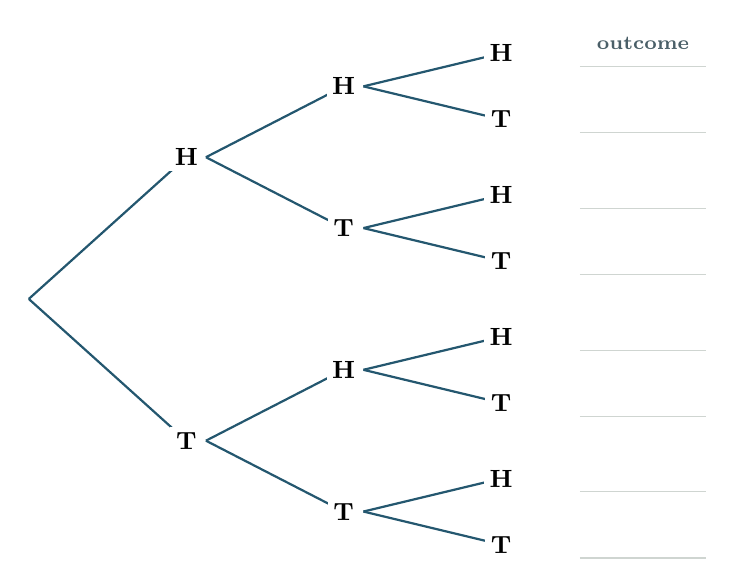
\begin{tikzpicture}[figstyle,font=\small,x=1cm,y=1cm]
  \foreach \s/\y in {H/1.8,T/-1.8}{\draw[chalkdk,thick](0,0)--(2,\y);\node[fill=white,inner sep=2pt,font=\small\bfseries]at(2,\y){\s};
    \foreach \t/\dy in {H/0.9,T/-0.9}{\draw[chalkdk,thick](2.25,\y)--(4,\y+\dy);\node[fill=white,inner sep=2pt,font=\small\bfseries]at(4,\y+\dy){\t};
      \foreach \u/\ddy in {H/0.42,T/-0.42}{\draw[chalkdk,thick](4.25,\y+\dy)--(6,\y+\dy+\ddy);\node[fill=white,inner sep=2pt,font=\small\bfseries]at(6,\y+\dy+\ddy){\u};
        \draw[line!150!white](7,\y+\dy+\ddy-0.17)--(8.6,\y+\dy+\ddy-0.17);}}}
  \node[font=\scriptsize\bfseries,inksoft]at(7.8,3.25){outcome};
\end{tikzpicture}\end{center}}
% Outcome grid for a two-step experiment. #1 row labels #2 column labels #3 cell size (cm)
% #4 1 = grey out the diagonal (selection without replacement) #5 drawing under the grid lines
% (shading, cell entries); cell (r,c) has its centre at (c+0.5, r+0.5)
\newcommand{\outgrid}[5]{\begin{center}\begin{tikzpicture}[figstyle,x=#3cm,y=-#3cm,font=\small]
  \foreach \l [count=\c] in {#2}{\node[font=\small\bfseries,chalkdk]at(\c+0.5,0.5){\l};\xdef\ncols{\c}}
  \foreach \l [count=\r] in {#1}{\node[font=\small\bfseries,chalkdk]at(0.5,\r+0.5){\l};\xdef\nrows{\r}}
  \ifnum#4=1 \foreach \i in {1,...,\nrows}{\fill[line!160!white](\i,\i)rectangle(\i+1,\i+1);
     \draw[inksoft!60](\i+0.25,\i+0.25)--(\i+0.75,\i+0.75)(\i+0.25,\i+0.75)--(\i+0.75,\i+0.25);}\fi
  #5
  \foreach \x in {2,...,\ncols}{\draw[chalkdk!55](\x,1)--(\x,\nrows+1);}
  \foreach \y in {2,...,\nrows}{\draw[chalkdk!55](1,\y)--(\ncols+1,\y);}
  \draw[chalkdk,thick](1,1)rectangle(\ncols+1,\nrows+1);
  \node[font=\scriptsize,inksoft,align=center]at(0.5,0.5){1st\,$\downarrow$\\2nd\,$\rightarrow$};
\end{tikzpicture}\end{center}}
% Counting boxes. #1 comma list of entries (leave an entry empty for a blank box) #2 label under each box
\newcommand{\slots}[2]{\begin{center}\begin{tikzpicture}[figstyle,font=\small]
  \foreach \v [count=\i] in {#1}{\draw[chalkdk,thick](1.9*\i-0.55,-0.55)rectangle(1.9*\i+0.55,0.55);\node[font=\large]at(1.9*\i,0){\v};\xdef\nslots{\i}}
  \foreach \v [count=\i] in {#2}{\node[font=\scriptsize,inksoft]at(1.9*\i,-0.85){\v};}
  \foreach \i in {2,...,\nslots}{\node[font=\large,chalkdk]at(1.9*\i-0.95,0){$\times$};}
\end{tikzpicture}\end{center}}

\begin{document}
\thispagestyle{empty}
\begin{tikzpicture}[remember picture,overlay]
  \fill[chalk] (current page.north west) rectangle ([yshift=-62mm]current page.north east);
  \node[anchor=north west,text=white,align=left] at ([xshift=20mm,yshift=-20mm]current page.north west)
    {{\Huge\bfseries\textsf{Chapter 8: Probability}}\\[4mm]{\LARGE\textsf{Student Question Booklet}}\\[3mm]{\large\textsf{Sections 8A--8J : Year 10 Mathematical Methods : 2026}}};
\end{tikzpicture}
\vspace{58mm}

\vspace{6mm}
\begin{refbox}
{\bfseries\color{chalkdk}How to use this booklet}\\[2pt]
This booklet is your \textbf{map through sections 8A--8J} --- Venn diagrams and two-way tables, the addition rule, conditional probability, arrays, tree diagrams, independence and, for 10A, counting arrangements and selections. For every section you will find:
\begin{itemize}[leftmargin=16pt,itemsep=2pt,topsep=3pt]
  \item \textbf{Worked examples} --- fully solved examples with a diagram where it helps, plus the matching textbook example numbers and pages to cross-reference.
  \item \textbf{Question sets} --- the questions to practise, grouped by \textit{Building Understanding}, \textit{Fluency}, \textit{Problem-solving}, \textit{Reasoning} and \textit{Enrichment}, with page numbers. Find them in your own textbook.
  \item \textbf{Hurdle questions} --- five questions you \textbf{must} be able to do to pass the section, with working space (and a diagram wherever you need to draw or complete one).
\end{itemize}
\vspace{2pt}{\small\color{inksoft}Diagrams are schematic (not to scale). Sections marked \textsf{10A} are extension. Give probabilities as fractions in simplest form, or as decimals when the question uses decimals. Always show working --- write the rule or draw the diagram before you calculate.}
\end{refbox}
\vspace{4mm}{\small\color{inksoft}Page references are to \emph{Essential Mathematics for the Victorian Curriculum 10 \& 10A}, 3rd ed. Question sets belong to the textbook; the worked examples, diagrams and hurdle questions are original material written for this course. Section 8K is not part of this course.}
\clearpage
\newpage
\quad
\clearpage

% =====================================================================
\sectionband{8A}{Review of probability}{CONSOLIDATING}

\begin{refbox}
{\bfseries\color{chalkdk}Textbook worked examples}\;\textcolor{inksoft}{\small(cross-reference in your textbook)}\\[3pt]
\begin{itemize}[leftmargin=16pt,itemsep=1pt,topsep=2pt]
  \item \textbf{Example 1} --- Calculating simple theoretical probabilities \textcolor{inksoft}{(p.\,684)}
  \item \textbf{Example 2} --- Calculating simple experimental probabilities \textcolor{inksoft}{(p.\,684)}
\end{itemize}
\vspace{4pt}{\bfseries\color{chalkdk}Question sets}\;\textcolor{inksoft}{\small(practise from your textbook)}\\[3pt]
\begin{itemize}[leftmargin=16pt,itemsep=1pt,topsep=2pt]
  \item \textbf{Building Understanding:} Q1--3 \textcolor{inksoft}{(p.\,683)}
  \item \textbf{Fluency:} Q1--5 \textcolor{inksoft}{(p.\,685--686)}
  \item \textbf{Problem-solving:} Q6--9 \textcolor{inksoft}{(p.\,686--687)}
  \item \textbf{Reasoning:} Q10--12 \textcolor{inksoft}{(p.\,687)}
  \item \textbf{Enrichment: Target probability:} Q13 \textcolor{inksoft}{(p.\,687)}
\end{itemize}\end{refbox}

\workedhead

\begin{worked}{Theoretical probability from a spinner}
The spinner below has eight equal sectors. Find:
\begin{parts}
  \item $\Pr(3)$
  \item $\Pr(\text{an even number})$
  \item $\Pr(\text{not } 3)$
  \item $\Pr(\text{a number greater than } 3)$.
\end{parts}
\spinner{8}{1,2,2,3,3,3,4,5}
\solution All eight sectors are equally likely, so
\[\Pr(\text{event})=\frac{\text{number of favourable sectors}}{8}.\]
\solp{a} Three sectors show $3$: $\Pr(3)=\dfrac38$.
\solp{b} The even sectors are $2, 2, 4$: $\Pr(\text{even})=\dfrac38$.
\solp{c} $\Pr(\text{not } 3) = 1-\Pr(3) = 1-\dfrac38=\dfrac58$.
\solp{d} The sectors $4$ and $5$ are greater than $3$: $\Pr(\text{greater than } 3)=\dfrac28=\dfrac14$.
\end{worked}

\begin{worked}{Experimental probability from a frequency table}
A die is rolled $200$ times to test whether it is fair.
\begin{center}\renewcommand{\arraystretch}{1.3}
\begin{tabular}{|l|c|c|c|c|c|c|}\hline
\textbf{Outcome} & 1 & 2 & 3 & 4 & 5 & 6 \\\hline
\textbf{Frequency} & 28 & 31 & 30 & 33 & 26 & 52 \\\hline
\end{tabular}\end{center}
\begin{parts}
  \item Find the experimental probability of rolling a $6$.
  \item Find the experimental probability of rolling an odd number.
  \item Does the die appear to be fair? Explain.
  \item Using these results, how many 6s would you expect in $500$ rolls?
\end{parts}
\solution Experimental probability is found from the results:
\[\text{experimental probability}=\frac{\text{number of times the event happened}}{\text{total number of trials}}.\]
\solp{a} $\Pr(6)=\dfrac{52}{200}=0.26$.
\solp{b} Odd numbers: $28+30+26=84$, so $\Pr(\text{odd})=\dfrac{84}{200}=0.42$.
\solp{c} For a fair die, $\Pr(6)=\dfrac16\approx0.17$. Over $200$ rolls we would expect about $33$ sixes, not $52$, so the die appears to be \textbf{biased towards 6}.
\solp{d} $0.26\times500=130$ sixes.
\end{worked}

\closepart{\notesfill}

\begin{hurdles}{8A}

\begin{hurdle}
A letter is chosen at random from the word \textbf{MISSISSIPPI}. Find:
\begin{parts}
  \item $\Pr(\text{S})$
  \item $\Pr(\text{a vowel})$
  \item $\Pr(\text{not P})$.
\end{parts}
\worklines{4}
\end{hurdle}

\begin{hurdle}
The spinner below has ten equal sectors.
\spinner{10}{1,1,1,2,2,3,4,4,5,6}
\begin{parts}
  \item Find $\Pr(1)$.
  \item Find $\Pr(\text{an even number})$.
  \item Find $\Pr(\text{a number less than } 4)$.
  \item How many 4s would you expect in $50$ spins?
\end{parts}
\worklines{4}
\end{hurdle}

\begin{hurdle}
A traffic survey counted the passengers (not including the driver) in $120$ cars.
\begin{center}\renewcommand{\arraystretch}{1.3}
\begin{tabular}{|l|c|c|c|c|c|}\hline
\textbf{Number of passengers} & 0 & 1 & 2 & 3 & 4 \\\hline
\textbf{Number of cars} & 54 & 38 & 17 & 8 & 3 \\\hline
\end{tabular}\end{center}
\begin{parts}
  \item Find the experimental probability that a car has exactly one passenger.
  \item Find the experimental probability that a car has at least two passengers.
  \item Estimate how many of the next $600$ cars will have no passengers.
\end{parts}
\worklines{4}
\end{hurdle}

\begin{hurdle}
A bag contains only red, blue and green counters. A counter is chosen at random. $\Pr(\text{red})=0.35$ and $\Pr(\text{blue})=0.4$.
\begin{parts}
  \item Find $\Pr(\text{green})$.
  \item Find $\Pr(\text{not blue})$.
  \item The bag holds $60$ counters. How many of each colour are there?
\end{parts}
\worklines{4}
\end{hurdle}

\begin{hurdle}
A fair 12-sided die, numbered $1$ to $12$, is rolled once. Find:
\begin{parts}
  \item $\Pr(\text{a prime number})$
  \item $\Pr(\text{a multiple of } 3 \text{ or a multiple of } 4)$
  \item $\Pr(\text{a number greater than } 12)$, and describe this event in words.
\end{parts}
\worklines{5}
\end{hurdle}

\end{hurdles}
\closepart{\linesfill}

% =====================================================================
\sectionband{8B}{Set notation in Venn diagrams and two-way tables}{CORE}

\begin{refbox}
{\bfseries\color{chalkdk}Textbook worked examples}\;\textcolor{inksoft}{\small(cross-reference in your textbook)}\\[3pt]
\begin{itemize}[leftmargin=16pt,itemsep=1pt,topsep=2pt]
  \item \textbf{Example 3} --- Listing sets \textcolor{inksoft}{(p.\,690)}
  \item \textbf{Example 4} --- Using Venn diagrams \textcolor{inksoft}{(p.\,691)}
  \item \textbf{Example 5} --- Using two-way tables \textcolor{inksoft}{(p.\,692)}
\end{itemize}
\vspace{4pt}{\bfseries\color{chalkdk}Question sets}\;\textcolor{inksoft}{\small(practise from your textbook)}\\[3pt]
\begin{itemize}[leftmargin=16pt,itemsep=1pt,topsep=2pt]
  \item \textbf{Building Understanding:} Q1--3 \textcolor{inksoft}{(p.\,689)}
  \item \textbf{Fluency:} Q1--6 \textcolor{inksoft}{(p.\,693--694)}
  \item \textbf{Problem-solving:} Q7--10 \textcolor{inksoft}{(p.\,694--695)}
  \item \textbf{Reasoning:} Q11--13 \textcolor{inksoft}{(p.\,695)}
  \item \textbf{Enrichment: Triple Venn diagrams:} Q14--15 \textcolor{inksoft}{(p.\,696)}
\end{itemize}\end{refbox}

\workedhead

\begin{worked}{Listing sets and drawing the Venn diagram}
Let $\xi=\{1,2,3,\ldots,12\}$, $A=\{\text{multiples of } 3\}$ and $B=\{\text{even numbers}\}$.
\begin{parts}
  \item List $A\cap B$, $A\cup B$ and $A'$.
  \item Show the elements on a Venn diagram.
  \item A number is chosen at random from $\xi$. Find $\Pr(A\cup B)$.
\end{parts}
\solution
\solp{a} $A=\{3,6,9,12\}$ and $B=\{2,4,6,8,10,12\}$, so\\
$A\cap B$ (in $A$ \emph{and} $B$) $=\{6,12\}$\\
$A\cup B$ (in $A$ \emph{or} $B$ or both) $=\{2,3,4,6,8,9,10,12\}$\\
$A'$ (not in $A$) $=\{1,2,4,5,7,8,10,11\}$.
\solp{b} Fill the overlap first, then the rest of each circle, then the numbers in neither set.
\venn{$A$}{$B$}{$3,\ 9$}{$6$\\$12$}{$2,\ 4$\\$8,\ 10$}{$1,\ 5,\ 7,\ 11$}
\solp{c} $n(A\cup B)=8$, so $\Pr(A\cup B)=\dfrac{8}{12}=\dfrac23$.
\end{worked}

\begin{worked}{From a Venn diagram to a two-way table}
In a class of $28$ students, $16$ play a team sport ($S$), $12$ play a musical instrument ($M$) and $5$ do both. Draw a Venn diagram and a two-way table, then find the probability that a randomly chosen student does exactly one of the two activities.
\venn{$S$}{$M$}{$11$}{$5$}{$7$}{$5$}
\begin{center}\renewcommand{\arraystretch}{1.3}
\begin{tabular}{|l|c|c|c|}\hline
 & $M$ & $M'$ & \textbf{Total} \\\hline
$S$ & $5$ & $11$ & $16$ \\\hline
$S'$ & $7$ & $5$ & $12$ \\\hline
\textbf{Total} & $12$ & $16$ & $28$ \\\hline
\end{tabular}\end{center}
\solution Start with the overlap: $5$. Then sport only $=16-5=11$, instrument only $=12-5=7$ and neither $=28-(11+5+7)=5$. In the table, each row and column must add to its total.\par
Exactly one activity means \emph{sport only} or \emph{instrument only}: $\Pr(\text{exactly one})=\dfrac{11+7}{28}=\dfrac{18}{28}=\dfrac{9}{14}$.
\end{worked}

\closepart{\notesfill}

\begin{hurdles}{8B}

\begin{hurdle}
Let $\xi=\{1,2,3,\ldots,15\}$, $A=\{\text{factors of } 12\}$ and $B=\{\text{odd numbers}\}$.
\begin{parts}
  \item List the elements of $A$, $A\cap B$ and $B'$.
  \item Complete the Venn diagram.
  \item Find $n(A\cup B)$.
  \item A number is chosen at random from $\xi$. Find $\Pr(A\cap B')$.
\end{parts}
\venn{$A$}{$B$}{}{}{}{}
\worklines{4}
\end{hurdle}

\begin{hurdle}
Of $40$ Year 10 students, $24$ have a part-time job ($J$), $18$ have a learner permit ($L$) and $9$ have both.
\begin{parts}
  \item Complete the Venn diagram.
  \item Find $\Pr(\text{learner permit only})$.
  \item Find $\Pr(J\cup L)$.
  \item Find $\Pr(\text{neither})$.
\end{parts}
\venn{$J$}{$L$}{}{}{}{}
\worklines{4}
\end{hurdle}

\begin{hurdle}
Sixty people were asked whether they own a cat ($C$) and whether they own a dog ($D$).
\begin{parts}
  \item Complete the two-way table.
  \item Find $\Pr(C\cap D')$.
  \item Find $\Pr(D)$.
  \item Find $\Pr(C'\cap D')$.
\end{parts}
\begin{center}\renewcommand{\arraystretch}{1}
\begin{tabular}{|>{\centering\arraybackslash}m{20mm}|>{\centering\arraybackslash}m{24mm}|>{\centering\arraybackslash}m{24mm}|>{\centering\arraybackslash}m{24mm}|}\hline
\rule{0pt}{6mm} & $D$ & $D'$ & \textbf{Total} \\\hline
\rule[-5mm]{0pt}{12mm}$C$ & $8$ & & $20$ \\\hline
\rule[-5mm]{0pt}{12mm}$C'$ & & & \\\hline
\rule[-5mm]{0pt}{12mm}\textbf{Total} & $26$ & & $60$ \\\hline
\end{tabular}\end{center}
\worklines{3}
\end{hurdle}

\begin{hurdle}
The Venn diagram shows the number of elements in events $A$ and $B$.
\venn{$A$}{$B$}{$6$}{$4$}{$9$}{$11$}
\begin{parts}
  \item Show the same information in a two-way table.
  \item Find $\Pr(A')$, $\Pr(A\cap B')$ and $\Pr(A\cup B)$.
\end{parts}
\worklines{5}
\end{hurdle}

\begin{hurdle}
Write the shaded region of each Venn diagram in set notation.
\begin{center}
\begin{tabular}{ccc}
\vennshade{\shadeAonly} & \vennshade{\shadeNeither} & \vennshade{\shadeBnotA} \\[2pt]
\textbf{(a)}\ \underline{\hspace{30mm}} & \textbf{(b)}\ \underline{\hspace{30mm}} & \textbf{(c)}\ \underline{\hspace{30mm}}
\end{tabular}
\end{center}
\worklines{2}
\end{hurdle}

\end{hurdles}
\closepart{\linesfill}

% =====================================================================
\sectionband{8C}{The addition rule}{CORE}

\begin{refbox}
{\bfseries\color{chalkdk}Textbook worked examples}\;\textcolor{inksoft}{\small(cross-reference in your textbook)}\\[3pt]
\begin{itemize}[leftmargin=16pt,itemsep=1pt,topsep=2pt]
  \item \textbf{Example 6} --- Applying the addition rule \textcolor{inksoft}{(p.\,698)}
  \item \textbf{Example 7} --- Using the addition rule \textcolor{inksoft}{(p.\,700)}
\end{itemize}
\vspace{4pt}{\bfseries\color{chalkdk}Question sets}\;\textcolor{inksoft}{\small(practise from your textbook)}\\[3pt]
\begin{itemize}[leftmargin=16pt,itemsep=1pt,topsep=2pt]
  \item \textbf{Building Understanding:} Q1--3 \textcolor{inksoft}{(p.\,698)}
  \item \textbf{Fluency:} Q1--5 \textcolor{inksoft}{(p.\,700--701)}
  \item \textbf{Problem-solving:} Q6--9 \textcolor{inksoft}{(p.\,701--702)}
  \item \textbf{Reasoning:} Q10--12 \textcolor{inksoft}{(p.\,702)}
  \item \textbf{Enrichment: Divisibility and the addition rule:} Q13--14 \textcolor{inksoft}{(p.\,702)}
\end{itemize}\end{refbox}

\workedhead

\begin{worked}{The addition rule with counting}
A number is chosen at random from $1$ to $30$. Let $A$ be ``a multiple of $4$'' and $B$ be ``a multiple of $6$''. Use the addition rule to find $\Pr(A\cup B)$, then check by listing.
\[\Pr(A\cup B)=\Pr(A)+\Pr(B)-\Pr(A\cap B)\]
\solution $A=\{4,8,12,16,20,24,28\}$, so $\Pr(A)=\dfrac{7}{30}$.\par
$B=\{6,12,18,24,30\}$, so $\Pr(B)=\dfrac{5}{30}$.\par
The numbers in both are the multiples of $12$: $A\cap B=\{12,24\}$, so $\Pr(A\cap B)=\dfrac{2}{30}$.
\[\Pr(A\cup B)=\frac{7}{30}+\frac{5}{30}-\frac{2}{30}=\frac{10}{30}=\frac13.\]
\textbf{Check:} $A\cup B=\{4,6,8,12,16,18,20,24,28,30\}$ has $10$ elements. We subtract $\Pr(A\cap B)$ because $12$ and $24$ were counted once in $A$ and again in $B$.
\end{worked}

\begin{worked}{The addition rule with given probabilities}
For two events, $\Pr(A)=0.45$, $\Pr(B)=0.3$ and $\Pr(A\cup B)=0.6$.
\begin{parts}
  \item Find $\Pr(A\cap B)$.
  \item Find $\Pr(A\cap B')$.
  \item Find $\Pr\big((A\cup B)'\big)$.
  \item Show all four regions on a Venn diagram.
\end{parts}
\solution
\solp{a} Rearrange the addition rule: $\Pr(A\cap B)=\Pr(A)+\Pr(B)-\Pr(A\cup B)=0.45+0.3-0.6=0.15$.
\solp{b} $A$ only: $\Pr(A\cap B')=\Pr(A)-\Pr(A\cap B)=0.45-0.15=0.3$.
\solp{c} Neither: $\Pr\big((A\cup B)'\big)=1-\Pr(A\cup B)=1-0.6=0.4$.
\solp{d} $B$ only is $0.3-0.15=0.15$. Check: $0.3+0.15+0.15+0.4=1$.
\venn{$A$}{$B$}{$0.3$}{$0.15$}{$0.15$}{$0.4$}
\textbf{Mutually exclusive} events have $\Pr(A\cap B)=0$, and then $\Pr(A\cup B)=\Pr(A)+\Pr(B)$.
\end{worked}

\closepart{\notesfill}

\begin{hurdles}{8C}

\begin{hurdle}
A number is chosen at random from $1$ to $40$. Let $A$ be ``a multiple of $5$'' and $B$ be ``a multiple of $8$''.
\begin{parts}
  \item Find $\Pr(A)$, $\Pr(B)$ and $\Pr(A\cap B)$.
  \item Use the addition rule to find $\Pr(A\cup B)$.
\end{parts}
\worklines{5}
\end{hurdle}

\begin{hurdle}
For two events, $\Pr(A)=0.6$, $\Pr(B)=0.5$ and $\Pr(A\cap B)=0.25$.
\begin{parts}
  \item Complete the Venn diagram with probabilities.
  \item Find $\Pr(A\cup B)$.
  \item Find $\Pr(A')$.
  \item Find $\Pr(A\cap B')$.
  \item Find the probability that neither event occurs.
\end{parts}
\venn{$A$}{$B$}{}{}{}{}
\worklines{3}
\end{hurdle}

\begin{hurdle}
For two events, $\Pr(A)=0.35$, $\Pr(B)=0.4$ and $\Pr(A\cup B)=0.75$. Are $A$ and $B$ mutually exclusive? Use the addition rule to explain.
\worklines{4}
\end{hurdle}

\begin{hurdle}
In a group of $50$ students, $22$ study French, $19$ study Japanese and $8$ study both. A student is chosen at random. Find the probability that the student studies:
\begin{parts}
  \item French or Japanese
  \item neither language
  \item exactly one of the two languages.
\end{parts}
\worklines{5}
\end{hurdle}

\begin{hurdle}
For two events, $\Pr(A)=0.7$ and $\Pr(B)=0.5$. A student writes $\Pr(A\cup B)=0.7+0.5=1.2$.
\begin{parts}
  \item Explain why this answer must be wrong, and what it tells you about $A$ and $B$.
  \item If in fact $\Pr(A\cup B)=0.9$, find $\Pr(A\cap B)$.
\end{parts}
\worklines{5}
\end{hurdle}

\end{hurdles}
\closepart{\linesfill}

% =====================================================================
\sectionband{8D}{Conditional probability}{CORE}

\begin{refbox}
{\bfseries\color{chalkdk}Textbook worked examples}\;\textcolor{inksoft}{\small(cross-reference in your textbook)}\\[3pt]
\begin{itemize}[leftmargin=16pt,itemsep=1pt,topsep=2pt]
  \item \textbf{Example 8} --- Finding conditional probabilities using a Venn diagram \textcolor{inksoft}{(p.\,704)}
  \item \textbf{Example 9} --- Finding conditional probabilities using a two-way table \textcolor{inksoft}{(p.\,705)}
\end{itemize}
\vspace{4pt}{\bfseries\color{chalkdk}Question sets}\;\textcolor{inksoft}{\small(practise from your textbook)}\\[3pt]
\begin{itemize}[leftmargin=16pt,itemsep=1pt,topsep=2pt]
  \item \textbf{Building Understanding:} Q1--3 \textcolor{inksoft}{(p.\,704)}
  \item \textbf{Fluency:} Q1--4 \textcolor{inksoft}{(p.\,706--707)}
  \item \textbf{Problem-solving:} Q5--8 \textcolor{inksoft}{(p.\,707)}
  \item \textbf{Reasoning:} Q9--11 \textcolor{inksoft}{(p.\,708)}
  \item \textbf{Enrichment: Investment workshops:} Q12 \textcolor{inksoft}{(p.\,708)}
\end{itemize}\end{refbox}

\workedhead

\begin{worked}{Conditional probability from a Venn diagram}
The Venn diagram shows the number of elements in events $A$ and $B$. Find:
\begin{parts}
  \item $\Pr(A\,|\,B)$
  \item $\Pr(B\,|\,A)$
  \item $\Pr(A)$.
\end{parts}
\venn{$A$}{$B$}{$7$}{$3$}{$5$}{$5$}
\solution $\Pr(A\,|\,B)$ means ``the probability of $A$, \emph{given} that $B$ has happened''. Knowing $B$ happened shrinks the sample space to the circle $B$.
\solp{a} $n(B)=3+5=8$, and $3$ of those are also in $A$: $\Pr(A\,|\,B)=\dfrac{n(A\cap B)}{n(B)}=\dfrac38$.
\solp{b} $n(A)=7+3=10$: $\Pr(B\,|\,A)=\dfrac{n(A\cap B)}{n(A)}=\dfrac{3}{10}$.
\solp{c} There are $7+3+5+5=20$ elements in total: $\Pr(A)=\dfrac{10}{20}=\dfrac12$.\par
\vspace{4pt}Note that $\Pr(A\,|\,B)\neq\Pr(B\,|\,A)$: the ``given'' event decides the denominator.
\end{worked}

\begin{worked}{Conditional probability from a two-way table}
A survey of $120$ students recorded whether each wears glasses ($G$) and whether each is left-handed ($L$).
\begin{center}\renewcommand{\arraystretch}{1.3}
\begin{tabular}{|l|c|c|c|}\hline
 & $L$ & $L'$ & \textbf{Total} \\\hline
$G$ & $6$ & $30$ & $36$ \\\hline
$G'$ & $10$ & $74$ & $84$ \\\hline
\textbf{Total} & $16$ & $104$ & $120$ \\\hline
\end{tabular}\end{center}
Find:
\begin{parts}
  \item $\Pr(G\,|\,L)$
  \item $\Pr(L\,|\,G)$.
\end{parts}
\solution
\solp{a} Given $L$: use the $L$ \emph{column} only ($16$ students), of whom $6$ wear glasses: $\Pr(G\,|\,L)=\dfrac{6}{16}=\dfrac38$. The rule gives the same result:
\[\Pr(G\,|\,L)=\frac{\Pr(G\cap L)}{\Pr(L)}=\frac{6/120}{16/120}=\frac{6}{16}=\frac38.\]
\solp{b} Given $G$: use the $G$ \emph{row} only ($36$ students): $\Pr(L\,|\,G)=\dfrac{6}{36}=\dfrac16$.
\end{worked}

\closepart{\notesfill}

\begin{hurdles}{8D}

\begin{hurdle}
The Venn diagram shows the number of elements in events $A$ and $B$.
\venn{$A$}{$B$}{$9$}{$6$}{$4$}{$6$}
Find:
\begin{parts}
  \item $\Pr(A\,|\,B)$
  \item $\Pr(B\,|\,A)$
  \item $\Pr(A'\,|\,B)$
  \item $\Pr(B\,|\,A')$.
\end{parts}
\worklines{4}
\end{hurdle}

\begin{hurdle}
Eighty people were asked whether they like coffee ($C$) and whether they like tea ($T$).
\begin{center}\renewcommand{\arraystretch}{1.3}
\begin{tabular}{|l|c|c|c|}\hline
 & $T$ & $T'$ & \textbf{Total} \\\hline
$C$ & $18$ & $34$ & $52$ \\\hline
$C'$ & $20$ & $8$ & $28$ \\\hline
\textbf{Total} & $38$ & $42$ & $80$ \\\hline
\end{tabular}\end{center}
Find:
\begin{parts}
  \item $\Pr(C\,|\,T)$
  \item $\Pr(T\,|\,C)$
  \item $\Pr(C'\,|\,T')$.
\end{parts}
\worklines{4}
\end{hurdle}

\begin{hurdle}
For two events, $\Pr(A)=0.5$, $\Pr(B)=0.4$ and $\Pr(A\cap B)=0.1$. Use $\Pr(A\,|\,B)=\dfrac{\Pr(A\cap B)}{\Pr(B)}$ to find:
\begin{parts}
  \item $\Pr(A\,|\,B)$
  \item $\Pr(B\,|\,A)$.
\end{parts}
\worklines{4}
\end{hurdle}

\begin{hurdle}
For two events, $\Pr(A\,|\,B)=0.3$ and $\Pr(B)=0.6$.
\begin{parts}
  \item Find $\Pr(A\cap B)$.
  \item If $\Pr(A)=0.45$, find $\Pr(B\,|\,A)$.
\end{parts}
\worklines{5}
\end{hurdle}

\begin{hurdle}
In a group of $30$ students, $12$ play soccer ($S$), $15$ play basketball ($B$) and $4$ play both.
\begin{parts}
  \item Complete the Venn diagram.
  \item A student chosen at random plays basketball. Find the probability that they also play soccer.
  \item A student chosen at random plays soccer. Find the probability that they also play basketball.
\end{parts}
\venn{$S$}{$B$}{}{}{}{}
\worklines{3}
\end{hurdle}

\end{hurdles}
\closepart{\linesfill}

% =====================================================================
\sectionband{8E}{Two-step experiments using arrays}{CORE}

\begin{refbox}
{\bfseries\color{chalkdk}Textbook worked examples}\;\textcolor{inksoft}{\small(cross-reference in your textbook)}\\[3pt]
\begin{itemize}[leftmargin=16pt,itemsep=1pt,topsep=2pt]
  \item \textbf{Example 10} --- Constructing a table with replacement \textcolor{inksoft}{(p.\,710)}
  \item \textbf{Example 11} --- Constructing a table without replacement \textcolor{inksoft}{(p.\,712)}
\end{itemize}
\vspace{4pt}{\bfseries\color{chalkdk}Question sets}\;\textcolor{inksoft}{\small(practise from your textbook)}\\[3pt]
\begin{itemize}[leftmargin=16pt,itemsep=1pt,topsep=2pt]
  \item \textbf{Building Understanding:} Q1--2 \textcolor{inksoft}{(p.\,710)}
  \item \textbf{Fluency:} Q1--4 \textcolor{inksoft}{(p.\,713)}
  \item \textbf{Problem-solving:} Q5--7 \textcolor{inksoft}{(p.\,714)}
  \item \textbf{Reasoning:} Q8--10 \textcolor{inksoft}{(p.\,714--715)}
  \item \textbf{Enrichment: Random weights:} Q11 \textcolor{inksoft}{(p.\,715)}
\end{itemize}\end{refbox}

\workedhead

\begin{worked}{An array with replacement}
Two fair four-sided dice, each numbered $1$ to $4$, are rolled and the numbers are added. Draw an array of the totals, then find:
\begin{parts}
  \item $\Pr(\text{total of } 5)$
  \item $\Pr(\text{total of } 7 \text{ or more})$
  \item $\Pr(\text{a double})$.
\end{parts}
\outgrid{1,2,3,4}{1,2,3,4}{0.8}{0}{%
  \foreach \r in {1,...,4}{\foreach \c in {1,...,4}{\pgfmathtruncatemacro{\s}{\r+\c}%
    \ifnum\s=5 \fill[amber!35](\c,\r)rectangle(\c+1,\r+1);\fi
    \node at(\c+0.5,\r+0.5){$\s$};}}}
\solution Each die can show any number on either roll, so the array has $4\times4=16$ equally likely outcomes.
\solp{a} A total of $5$ appears $4$ times (shaded): $\Pr(5)=\dfrac{4}{16}=\dfrac14$.
\solp{b} Totals of $7$ or more are $7, 7, 8$: $\Pr(7 \text{ or more})=\dfrac{3}{16}$.
\solp{c} The doubles lie on the diagonal ($1{+}1, 2{+}2, 3{+}3, 4{+}4$): $\Pr(\text{double})=\dfrac{4}{16}=\dfrac14$.
\end{worked}

\begin{worked}{An array without replacement}
Five cards numbered $1$ to $5$ are shuffled. Two cards are drawn, one after the other, \textbf{without replacement}. Find:
\begin{parts}
  \item $\Pr(\text{both even})$
  \item $\Pr(\text{the two cards add to } 6)$
  \item $\Pr(\text{at least one card is a } 5)$.
\end{parts}
\outgrid{1,2,3,4,5}{1,2,3,4,5}{0.8}{1}{%
  \foreach \r in {1,...,5}{\foreach \c in {1,...,5}{\ifnum\r=\c\else\pgfmathtruncatemacro{\s}{\r+\c}%
    \ifnum\s=6 \fill[amber!35](\c,\r)rectangle(\c+1,\r+1);\fi
    \node[font=\scriptsize]at(\c+0.5,\r+0.5){$\r,\!\c$};\fi}}}
\solution The first card cannot be drawn again, so the diagonal (the same card twice) is crossed out, leaving $5\times4=20$ outcomes.
\solp{a} Both even: $(2,4)$ and $(4,2)$, so $\Pr(\text{both even})=\dfrac{2}{20}=\dfrac1{10}$.
\solp{b} Total of $6$ (shaded): $(1,5), (5,1), (2,4), (4,2)$ --- but \emph{not} $(3,3)$ --- so $\Pr=\dfrac{4}{20}=\dfrac15$.
\solp{c} At least one $5$: the last row and the last column, $8$ outcomes, so $\Pr=\dfrac{8}{20}=\dfrac25$.
\end{worked}

\closepart{\notesfill}

\begin{hurdles}{8E}

\begin{hurdle}
A coin is tossed and a fair six-sided die is rolled.
\begin{parts}
  \item Complete the array of outcomes (for example, H3).
  \item Find $\Pr(\text{a head and an even number})$.
  \item Find $\Pr(\text{a tail and a number greater than } 4)$.
  \item Find $\Pr(\text{a head or a } 6)$.
\end{parts}
\outgrid{H,T}{1,2,3,4,5,6}{0.85}{0}{}
\worklines{3}
\end{hurdle}

\begin{hurdle}
Two fair six-sided dice are rolled and the numbers are added.
\begin{parts}
  \item Complete the array of totals.
  \item Find $\Pr(\text{total of } 7)$.
  \item Find $\Pr(\text{total of } 10 \text{ or more})$.
  \item Find $\Pr(\text{the total is a prime number})$.
\end{parts}
\outgrid{1,2,3,4,5,6}{1,2,3,4,5,6}{0.75}{0}{}
\worklines{3}
\end{hurdle}

\begin{hurdle}
Two letters are chosen at random, one after the other, \textbf{without replacement}, from the word \textbf{SQUARE}.
\begin{parts}
  \item Complete the array. How many outcomes are there?
  \item Find $\Pr(\text{both letters are vowels})$.
  \item Find $\Pr(\text{at least one letter is a vowel})$.
  \item Find $\Pr(\text{the first letter is S})$.
\end{parts}
\outgrid{S,Q,U,A,R,E}{S,Q,U,A,R,E}{0.75}{1}{}
\worklines{3}
\end{hurdle}

\begin{hurdle}
Two digits are chosen from $\{1,2,3\}$ to make a two-digit number (the first digit chosen is the tens digit).
\begin{parts}
  \item The digits are chosen \textbf{with} replacement.\\ List all the possible numbers, then find $\Pr(\text{greater than } 20)$ and $\Pr(\text{even})$.
  \item The digits are chosen \textbf{without} replacement.\\ List all the possible numbers, then find $\Pr(\text{even})$.
\end{parts}
\worklines{6}
\end{hurdle}

\begin{hurdle}
Explain why the diagonal of an array is crossed out when items are selected \textbf{without} replacement. Then find the number of outcomes when two items are chosen in order from $8$ different items:
\begin{parts}
  \item with replacement
  \item without replacement.
\end{parts}
\worklines{5}
\end{hurdle}

\end{hurdles}
\closepart{\linesfill}

% =====================================================================
\sectionband{8F}{Using tree diagrams}{CORE}

\begin{refbox}
{\bfseries\color{chalkdk}Textbook worked examples}\;\textcolor{inksoft}{\small(cross-reference in your textbook)}\\[3pt]
\begin{itemize}[leftmargin=16pt,itemsep=1pt,topsep=2pt]
  \item \textbf{Example 12} --- Constructing a tree diagram for multi-stage experiments \textcolor{inksoft}{(p.\,719)}
  \item \textbf{Example 13} --- Using a tree diagram for experiments without replacement \textcolor{inksoft}{(p.\,720)}
\end{itemize}
\vspace{4pt}{\bfseries\color{chalkdk}Question sets}\;\textcolor{inksoft}{\small(practise from your textbook)}\\[3pt]
\begin{itemize}[leftmargin=16pt,itemsep=1pt,topsep=2pt]
  \item \textbf{Building Understanding:} Q1--2 \textcolor{inksoft}{(p.\,718)}
  \item \textbf{Fluency:} Q1--4 \textcolor{inksoft}{(p.\,721--722)}
  \item \textbf{Problem-solving:} Q5--8 \textcolor{inksoft}{(p.\,723)}
  \item \textbf{Reasoning:} Q9--12 \textcolor{inksoft}{(p.\,724)}
  \item \textbf{Enrichment: Fermat and Pascal:} Q13 \textcolor{inksoft}{(p.\,725)}
\end{itemize}\end{refbox}

\workedhead

\begin{worked}{A tree diagram with replacement}
A bag holds $3$ red ($R$) and $2$ blue ($B$) counters. A counter is drawn, its colour noted, and it is \textbf{replaced}; then a second counter is drawn. Find:
\begin{parts}
  \item $\Pr(RR)$
  \item $\Pr(\text{one of each colour})$
  \item $\Pr(\text{at least one blue})$.
\end{parts}
\treetwo{$R$/\frac35/$R$/\frac35/$B$/\frac25}{$B$/\frac25/$R$/\frac35/$B$/\frac25}{1}{\frac{9}{25}/\frac{6}{25}/\frac{6}{25}/\frac{4}{25}}
\solution Because the counter is replaced, the second-stage probabilities are the same as the first. \textbf{Multiply along} a path, then \textbf{add} the paths you need.
\solp{a} $\Pr(RR)=\dfrac35\times\dfrac35=\dfrac{9}{25}$.
\solp{b} One of each: $\Pr(RB)+\Pr(BR)=\dfrac{6}{25}+\dfrac{6}{25}=\dfrac{12}{25}$.
\solp{c} At least one blue is everything except $RR$: $1-\Pr(RR)=1-\dfrac{9}{25}=\dfrac{16}{25}$.
\end{worked}

\begin{worked}{A tree diagram without replacement}
The same bag ($3$ red, $2$ blue) is used, but this time the first counter is \textbf{not} replaced. Find:
\begin{parts}
  \item $\Pr(RR)$
  \item $\Pr(\text{one of each colour})$
  \item $\Pr(BB)$.
\end{parts}
\treetwo{$R$/\frac35/$R$/\frac24/$B$/\frac24}{$B$/\frac25/$R$/\frac34/$B$/\frac14}{1}{\frac{6}{20}/\frac{6}{20}/\frac{6}{20}/\frac{2}{20}}
\solution After one counter is taken, only $4$ remain, so every second-stage denominator is $4$ --- and the numerators depend on what was taken first.
\solp{a} $\Pr(RR)=\dfrac35\times\dfrac24=\dfrac{6}{20}=\dfrac{3}{10}$.
\solp{b} One of each: $\Pr(RB)+\Pr(BR)=\dfrac{6}{20}+\dfrac{6}{20}=\dfrac{12}{20}=\dfrac35$.
\solp{c} $\Pr(BB)=\dfrac25\times\dfrac14=\dfrac{2}{20}=\dfrac1{10}$.\par
\vspace{4pt}\textbf{Check:} the outcomes cover everything, so $\dfrac{3}{10}+\dfrac35+\dfrac1{10}=1$.
\end{worked}

\closepart{\notesfill}

\begin{hurdles}{8F}

\begin{hurdle}
A biased coin lands heads ($H$) with probability $0.6$. It is tossed twice.
\begin{parts}
  \item Complete the tree diagram, including the probability of each outcome.
  \item Find $\Pr(HH)$.
  \item Find $\Pr(\text{exactly one head})$.
  \item Find $\Pr(\text{at least one tail})$.
\end{parts}
\treetwo{$H$/\blankp/$H$/\blankp/$T$/\blankp}{$T$/\blankp/$H$/\blankp/$T$/\blankp}{1}{\blankp/\blankp/\blankp/\blankp}
\worklines{3}
\end{hurdle}

\begin{hurdle}
A box holds $4$ green ($G$) and $6$ yellow ($Y$) tennis balls. Two balls are taken out \textbf{without replacement}.
\begin{parts}
  \item Complete the tree diagram.
  \item Find $\Pr(GG)$.
  \item Find $\Pr(\text{both balls are the same colour})$.
  \item Find $\Pr(\text{at least one green})$.
\end{parts}
\treetwo{$G$/\blankp/$G$/\blankp/$Y$/\blankp}{$Y$/\blankp/$G$/\blankp/$Y$/\blankp}{1}{\blankp/\blankp/\blankp/\blankp}
\worklines{3}
\end{hurdle}

\begin{hurdle}
The probability of rain on Monday is $0.3$. If it rains on Monday, the probability of rain on Tuesday is $0.6$. If it does not rain on Monday, the probability of rain on Tuesday is $0.2$.
\begin{parts}
  \item Draw a tree diagram for the two days.
  \item Find the probability that it rains on both days.
  \item Find the probability that it rains on exactly one of the two days.
  \item Find the probability that it rains on Tuesday.
\end{parts}
\worklines{7}
\end{hurdle}

\begin{hurdle}
A fair coin is tossed three times.
\begin{parts}
  \item Complete the tree diagram and list the eight outcomes.
  \item Find $\Pr(\text{exactly two heads})$.
  \item Find $\Pr(\text{at least one head})$.
\end{parts}
\treeHTthree
\worklines{3}
\end{hurdle}

\begin{hurdle}
A bag holds $5$ red and $3$ white marbles. Two are drawn \textbf{without replacement}. A student writes $\Pr(RR)=\dfrac58\times\dfrac58=\dfrac{25}{64}$.
\begin{parts}
  \item Explain the mistake.
  \item Find the correct value of $\Pr(RR)$.
\end{parts}
\worklines{5}
\end{hurdle}

\end{hurdles}
\closepart{\linesfill}

% =====================================================================
\sectionband{8G}{Independent events}{CORE}

\begin{refbox}
{\bfseries\color{chalkdk}Textbook worked examples}\;\textcolor{inksoft}{\small(cross-reference in your textbook)}\\[3pt]
\begin{itemize}[leftmargin=16pt,itemsep=1pt,topsep=2pt]
  \item \textbf{Example 14} --- Checking for independent events \textcolor{inksoft}{(p.\,730)}
\end{itemize}
\vspace{4pt}{\bfseries\color{chalkdk}Question sets}\;\textcolor{inksoft}{\small(practise from your textbook)}\\[3pt]
\begin{itemize}[leftmargin=16pt,itemsep=1pt,topsep=2pt]
  \item \textbf{Building Understanding:} Q1--3 \textcolor{inksoft}{(p.\,729)}
  \item \textbf{Fluency:} Q1--4 \textcolor{inksoft}{(p.\,731)}
  \item \textbf{Problem-solving:} Q5--7 \textcolor{inksoft}{(p.\,732)}
  \item \textbf{Reasoning:} Q8--9 \textcolor{inksoft}{(p.\,732)}
  \item \textbf{Enrichment: Independence and the addition rule:} Q10--11 \textcolor{inksoft}{(p.\,732)}
\end{itemize}\end{refbox}

\workedhead

\begin{worked}{Testing for independence by multiplying}
A number is chosen at random from $1$ to $12$. Let $A$ be ``an even number'' and $B$ be ``a multiple of $3$''. Are $A$ and $B$ independent?
\[A \text{ and } B \text{ are independent if } \Pr(A\cap B)=\Pr(A)\times\Pr(B) \quad\big(\text{equivalently } \Pr(A\,|\,B)=\Pr(A)\big).\]
\solution $\Pr(A)=\dfrac{6}{12}=\dfrac12$ and $\Pr(B)=\dfrac{4}{12}=\dfrac13$, so $\Pr(A)\times\Pr(B)=\dfrac16$.\par
Both even \emph{and} a multiple of $3$: $\{6,12\}$, so $\Pr(A\cap B)=\dfrac{2}{12}=\dfrac16$. The two are equal, so $A$ and $B$ \textbf{are independent}.\par
\textbf{Check with the other test:} given $B=\{3,6,9,12\}$, two of the four are even: $\Pr(A\,|\,B)=\dfrac24=\dfrac12=\Pr(A)$. Knowing $B$ happened does not change the chance of $A$.
\end{worked}

\begin{worked}{Testing for independence from a two-way table}
Fifty students were surveyed about their year level and whether they wear glasses ($G$).
\begin{center}\renewcommand{\arraystretch}{1.3}
\begin{tabular}{|l|c|c|c|}\hline
 & $G$ & $G'$ & \textbf{Total} \\\hline
Year 9 & $6$ & $14$ & $20$ \\\hline
Year 10 & $9$ & $21$ & $30$ \\\hline
\textbf{Total} & $15$ & $35$ & $50$ \\\hline
\end{tabular}\end{center}
Is wearing glasses independent of being in Year 9?\par
\solution $\Pr(G)=\dfrac{15}{50}=0.3$ and $\Pr(G\,|\,\text{Year 9})=\dfrac{6}{20}=0.3$ (use the Year 9 row only).\par
These are equal, so wearing glasses \textbf{is independent} of being in Year 9. (The Year 10 row agrees: $\dfrac{9}{30}=0.3$.)
\end{worked}

\closepart{\notesfill}

\begin{hurdles}{8G}

\begin{hurdle}
A number is chosen at random from $1$ to $20$. Let $A$ be ``an even number'' and $B$ be ``a multiple of $5$''.
\begin{parts}
  \item Find $\Pr(A)$, $\Pr(B)$ and $\Pr(A\cap B)$.
  \item Are $A$ and $B$ independent? Justify your answer.
\end{parts}
\worklines{5}
\end{hurdle}

\begin{hurdle}
A number is chosen at random from $1$ to $20$. Let $A$ be ``an even number'' and $C$ be ``a prime number''.
\begin{parts}
  \item Find $\Pr(C)$ and $\Pr(A\cap C)$.
  \item Are $A$ and $C$ independent? Justify your answer.
\end{parts}
\worklines{5}
\end{hurdle}

\begin{hurdle}
The Venn diagram shows the number of elements in events $A$ and $B$. Decide whether $A$ and $B$ are independent.
\venn{$A$}{$B$}{$6$}{$4$}{$6$}{$9$}
\worklines{4}
\end{hurdle}

\begin{hurdle}
$A$ and $B$ are independent events with $\Pr(A)=0.4$ and $\Pr(B)=0.5$.
\begin{parts}
  \item Find $\Pr(A\cap B)$.
  \item Find $\Pr(A\cup B)$.
  \item Find $\Pr(A'\cap B')$.
\end{parts}
\worklines{5}
\end{hurdle}

\begin{hurdle}
Eighty students were asked whether they walk to school ($W$).
\begin{center}\renewcommand{\arraystretch}{1.3}
\begin{tabular}{|l|c|c|c|}\hline
 & $W$ & $W'$ & \textbf{Total} \\\hline
Year 7 & $12$ & $28$ & $40$ \\\hline
Year 8 & $18$ & $22$ & $40$ \\\hline
\textbf{Total} & $30$ & $50$ & $80$ \\\hline
\end{tabular}\end{center}
Is walking to school independent of being in Year 7? Justify your answer.
\worklines{4}
\end{hurdle}

\end{hurdles}
\closepart{\linesfill}

% =====================================================================
\sectionband{8H}{Counting principles and factorial notation}{10A}

\begin{refbox}
{\bfseries\color{chalkdk}Textbook worked examples}\;\textcolor{inksoft}{\small(cross-reference in your textbook)}\\[3pt]
\begin{itemize}[leftmargin=16pt,itemsep=1pt,topsep=2pt]
  \item \textbf{Example 15} --- Using the addition and multiplication principles \textcolor{inksoft}{(p.\,734)}
  \item \textbf{Example 16} --- Evaluating factorials \textcolor{inksoft}{(p.\,735)}
\end{itemize}
\vspace{4pt}{\bfseries\color{chalkdk}Question sets}\;\textcolor{inksoft}{\small(practise from your textbook)}\\[3pt]
\begin{itemize}[leftmargin=16pt,itemsep=1pt,topsep=2pt]
  \item \textbf{Building Understanding:} Q1--2 \textcolor{inksoft}{(p.\,734)}
  \item \textbf{Fluency:} Q1--4 \textcolor{inksoft}{(p.\,735)}
  \item \textbf{Problem-solving:} Q5--8 \textcolor{inksoft}{(p.\,736)}
  \item \textbf{Reasoning:} Q9--11 \textcolor{inksoft}{(p.\,736)}
  \item \textbf{Enrichment: Proofs with factorials:} Q12--14 \textcolor{inksoft}{(p.\,736)}
\end{itemize}\end{refbox}

\workedhead

\begin{worked}{``Or'' adds, ``and'' multiplies}
A caf\'e sells $4$ hot drinks, $5$ cold drinks and $3$ cakes. How many ways can you choose:
\begin{parts}
  \item one drink
  \item one drink and one cake
  \item one hot drink and one cold drink?
\end{parts}
\solution
\solp{a} One drink is a hot drink \emph{or} a cold drink: \textbf{addition principle}, $4+5=9$ ways.
\solp{b} A drink \emph{and} a cake: \textbf{multiplication principle}, $9\times3=27$ ways (each of the $9$ drinks can go with each of the $3$ cakes).
\slots{9,3}{drink,cake}
\solp{c} A hot drink \emph{and} a cold drink: $4\times5=20$ ways.
\end{worked}

\begin{worked}{Working with factorials}
Evaluate without a calculator:
\begin{parts}
  \item $6!$
  \item $\dfrac{8!}{6!}$
  \item $\dfrac{10!}{7!\,3!}$
  \item Simplify $\dfrac{(n+1)!}{n!}$.
\end{parts}
\solution $n!=n\times(n-1)\times\cdots\times2\times1$, and $0!=1$.
\solp{a} $6!=6\times5\times4\times3\times2\times1=720$
\solp{b} $\dfrac{8!}{6!}=\dfrac{8\times7\times\cancel{6!}}{\cancel{6!}}=8\times7=56$
\solp{c} $\dfrac{10!}{7!\,3!}=\dfrac{10\times9\times8\times\cancel{7!}}{\cancel{7!}\times3\times2\times1}=\dfrac{720}{6}=120$
\solp{d} $\dfrac{(n+1)!}{n!}=\dfrac{(n+1)\times\cancel{n!}}{\cancel{n!}}=n+1$\par
\vspace{4pt}\textbf{Tip:} write the larger factorial down to the smaller one, then cancel.
\end{worked}

\closepart{\notesfill}

\begin{hurdles}{8H}

\begin{hurdle}
A school offers $5$ language electives and $7$ arts electives. How many ways can a student choose:
\begin{parts}
  \item one elective from either list
  \item one language elective and one arts elective?
\end{parts}
\worklines{4}
\end{hurdle}

\begin{hurdle}
A number plate has $3$ letters (A to Z) followed by $2$ digits ($0$ to $9$). Letters and digits may repeat. How many different number plates are possible?
\slots{,,,,}{letter,letter,letter,digit,digit}
\worklines{3}
\end{hurdle}

\begin{hurdle}
Evaluate without a calculator:
\begin{parts}
  \item $5!$
  \item $\dfrac{9!}{7!}$
  \item $\dfrac{7!}{4!\,3!}$
  \item $0!$
\end{parts}
\worklines{4}
\end{hurdle}

\begin{hurdle}
Simplify:
\begin{parts}
  \item $\dfrac{n!}{(n-1)!}$
  \item $\dfrac{(n+2)!}{n!}$
\end{parts}
\worklines{4}
\end{hurdle}

\begin{hurdle}
A code has $4$ characters. Each character is a digit ($0$ to $9$) or one of the letters A to F. How many codes are possible if:
\begin{parts}
  \item characters may repeat
  \item no character may be used more than once?
\end{parts}
\worklines{4}
\end{hurdle}

\end{hurdles}
\closepart{\linesfill}

% =====================================================================
\sectionband{8I}{Arrangements}{10A}

\begin{refbox}
{\bfseries\color{chalkdk}Textbook worked examples}\;\textcolor{inksoft}{\small(cross-reference in your textbook)}\\[3pt]
\begin{itemize}[leftmargin=16pt,itemsep=1pt,topsep=2pt]
  \item \textbf{Example 17} --- Finding the total number of arrangements \textcolor{inksoft}{(p.\,739)}
  \item \textbf{Example 18} --- Finding arrangements with restrictions \textcolor{inksoft}{(p.\,739)}
\end{itemize}
\vspace{4pt}{\bfseries\color{chalkdk}Question sets}\;\textcolor{inksoft}{\small(practise from your textbook)}\\[3pt]
\begin{itemize}[leftmargin=16pt,itemsep=1pt,topsep=2pt]
  \item \textbf{Building Understanding:} Q1--4 \textcolor{inksoft}{(p.\,738)}
  \item \textbf{Fluency:} Q1--5 \textcolor{inksoft}{(p.\,740)}
  \item \textbf{Problem-solving:} Q6--9 \textcolor{inksoft}{(p.\,740)}
  \item \textbf{Reasoning:} Q10--12 \textcolor{inksoft}{(p.\,741)}
  \item \textbf{Enrichment: How many numbers?:} Q13--15 \textcolor{inksoft}{(p.\,741)}
\end{itemize}\end{refbox}

\workedhead

\begin{worked}{Counting arrangements with boxes}
\begin{parts}
  \item In how many ways can $6$ different books be arranged on a shelf?
  \item Eight runners race. In how many ways can first, second and third place be filled?
\end{parts}
\solution Draw one box per position and fill it with the number of choices left.
\solp{a} $6\times5\times4\times3\times2\times1=6!=720$.
\solp{b} $8$ runners can come first, then $7$ are left for second, then $6$ for third: $8\times7\times6=336$.
\slots{8,7,6}{1st,2nd,3rd}
This is $\nPr{8}{3}=\dfrac{8!}{(8-3)!}=\dfrac{8!}{5!}=336$.
\end{worked}

\begin{worked}{Arrangements with restrictions}
The letters of the word \textbf{PRIME} are arranged in a row. How many arrangements:
\begin{parts}
  \item are there altogether
  \item begin with P
  \item begin and end with a vowel
  \item have the two vowels next to each other?
\end{parts}
\solution \textbf{Fill the restricted positions first.}
\solp{a} No restrictions: $5!=120$.
\solp{b} The first box must be P ($1$ way); the other $4$ letters fill the rest: $1\times4!=24$.
\solp{c} First box: $2$ vowels (I or E); last box: the $1$ vowel left; the $3$ consonants fill the middle: $2\times3\times2\times1\times1=12$.
\slots{2,3,2,1,1}{vowel,,,,vowel}
\solp{d} Glue I and E into one block: arrange $4$ items ($4!$), then arrange I and E inside the block ($2!$): $4!\times2!=48$.
\end{worked}

\closepart{\notesfill}

\begin{hurdles}{8I}

\begin{hurdle}
In how many ways can $7$ people stand in a queue?
\worklines{3}
\end{hurdle}

\begin{hurdle}
A club has $10$ members. In how many ways can a president, a vice-president and a secretary be chosen? Write your answer using $\nPr{n}{r}$ notation as well.
\slots{,,}{president,vice-pres.,secretary}
\worklines{3}
\end{hurdle}

\begin{hurdle}
The letters of the word \textbf{FRACTION} are arranged in a row. How many arrangements:
\begin{parts}
  \item are there altogether
  \item begin with F
  \item begin with a vowel?
\end{parts}
\worklines{5}
\end{hurdle}

\begin{hurdle}
Five friends, including Ana and Ben, sit in a row of five seats. In how many ways can they sit if:
\begin{parts}
  \item Ana and Ben must sit together
  \item Ana and Ben must \textbf{not} sit together?
\end{parts}
\worklines{5}
\end{hurdle}

\begin{hurdle}
Three-digit numbers are made from the digits $1, 2, 3, 4, 5, 6$, with no digit repeated. How many of these numbers:
\begin{parts}
  \item are there altogether
  \item are even
  \item are greater than $400$?
\end{parts}
\worklines{5}
\end{hurdle}

\end{hurdles}
\closepart{\linesfill}

% =====================================================================
\sectionband{8J}{Selections}{10A}

\begin{refbox}
{\bfseries\color{chalkdk}Textbook worked examples}\;\textcolor{inksoft}{\small(cross-reference in your textbook)}\\[3pt]
\begin{itemize}[leftmargin=16pt,itemsep=1pt,topsep=2pt]
  \item \textbf{Example 19} --- Evaluating $\nCr{n}{r}$ or $\binom{n}{r}$ \textcolor{inksoft}{(p.\,743)}
  \item \textbf{Example 20} --- Finding the number of possible selections \textcolor{inksoft}{(p.\,744)}
  \item \textbf{Example 21} --- Making selections from two groups \textcolor{inksoft}{(p.\,744)}
\end{itemize}
\vspace{4pt}{\bfseries\color{chalkdk}Question sets}\;\textcolor{inksoft}{\small(practise from your textbook)}\\[3pt]
\begin{itemize}[leftmargin=16pt,itemsep=1pt,topsep=2pt]
  \item \textbf{Building Understanding:} Q1--2 \textcolor{inksoft}{(p.\,742--743)}
  \item \textbf{Fluency:} Q1--5 \textcolor{inksoft}{(p.\,744--745)}
  \item \textbf{Problem-solving:} Q6--8 \textcolor{inksoft}{(p.\,745)}
  \item \textbf{Reasoning:} Q9--11 \textcolor{inksoft}{(p.\,745)}
  \item \textbf{Enrichment: Choosing any number of options:} Q12--14 \textcolor{inksoft}{(p.\,745)}
\end{itemize}\end{refbox}

\workedhead

\begin{worked}{Evaluating $\nCr{n}{r}$}
\begin{parts}
  \item Evaluate $\nCr{7}{3}$.
  \item Evaluate $\dbinom{10}{2}$.
  \item Explain why $\nCr{7}{3}=\nCr{7}{4}$.
\end{parts}
\[\nCr{n}{r}=\binom{n}{r}=\frac{n!}{r!\,(n-r)!}\]
\solution
\solp{a} $\nCr{7}{3}=\dfrac{7!}{3!\,4!}=\dfrac{7\times6\times5}{3\times2\times1}=\dfrac{210}{6}=35$
\solp{b} $\dbinom{10}{2}=\dfrac{10!}{2!\,8!}=\dfrac{10\times9}{2\times1}=45$
\solp{c} $\nCr{7}{4}=\dfrac{7!}{4!\,3!}$, which is the same expression as $\nCr{7}{3}$. Choosing the $3$ items to take is the same as choosing the $4$ items to leave behind.
\end{worked}

\begin{worked}{Selections from one group and from two groups}
\begin{parts}
  \item A committee of $3$ is chosen from $9$ people. How many committees are possible?
  \item A team of $2$ teachers and $3$ students is chosen from $5$ teachers and $6$ students. How many teams are possible?
\end{parts}
\solution In a committee the order does not matter, so this is a \textbf{selection}.
\solp{a} $\nCr{9}{3}=\dfrac{9\times8\times7}{3\times2\times1}=84$.
\solp{b} Choose the teachers \emph{and} the students, then multiply: $\nCr{5}{2}\times\nCr{6}{3}=10\times20=200$.
\end{worked}

\closepart{\notesfill}

\begin{hurdles}{8J}

\begin{hurdle}
Evaluate without a calculator:
\begin{parts}
  \item $\nCr{6}{2}$
  \item $\dbinom{8}{3}$
  \item $\nCr{12}{1}$
  \item $\nCr{5}{5}$
\end{parts}
\worklines{4}
\end{hurdle}

\begin{hurdle}
A pizza shop offers $10$ toppings. In how many ways can $4$ different toppings be chosen?
\worklines{3}
\end{hurdle}

\begin{hurdle}
A coach chooses a team of $5$ from a squad of $12$ players.
\begin{parts}
  \item How many teams are possible?
  \item How many of these teams include the captain?
\end{parts}
\worklines{4}
\end{hurdle}

\begin{hurdle}
A group of $3$ boys and $2$ girls is chosen from $7$ boys and $5$ girls. How many groups are possible?
\worklines{4}
\end{hurdle}

\begin{hurdle}
Two letters are chosen from A, B, C and D.
\begin{parts}
  \item List every \textbf{arrangement} (order matters) of two letters. How many are there?
  \item List every \textbf{selection} (order does not matter) of two letters. How many are there?
  \item Explain how the two answers are connected, using $2!$.
\end{parts}
\worklines{5}
\end{hurdle}

\end{hurdles}
\par\linesfill

\begin{center}\small\color{inksoft}\rule{0.5\linewidth}{0.3pt}\\[3pt]
End of Chapter 8 hurdle booklet --- check your working against the worked examples and ask in class if any hurdle question is unclear.
\end{center}
\end{document}
